\section{Vandermonde Matrix}

We start by presenting the background code and miscelaneous functions for matrices and linear algebra.

\lstinputlisting[caption={Code for the Matrix class used throughout this work}, linerange={11-47}]{matrix_class.py}
\lstinputlisting[caption={Matrix and vector multiplication functions, and a function to check if a solution x to the system of equations Ax = b is correct.}, linerange={63-68, 98-144}]{matrix_functions.py}
\lstinputlisting[caption={Code to import the data and apply the algorithms described throughout this section}, linerange={18-40, 73-108}]{vandermonde.py}

In this section we will work with a Vandermonde matrix $V$, which is defined as an $N$x$N$ matrix with elements $V_{i,j} = x_i^j$ for rows $i$ and columns $j$ ranging from $0$ to $N-1$. For any set with N $(x_i, y_i)$ points, we can populate the Vandermonde matrix and solve the set of linear equations $Vc = y$ to find the coefficients $c$ of the unique polynomial passing through all $(x_i, y_i)$ points. Here, we will apply two different methods to find this polynomial and compare the results. 
\\ \\
We will begin by introducing both methods, and providing the code used to implement them in Python. Afterwards we present the results of our implementation, and a discussion of these results.

\subsection{LU Decomposition}

Solving an equation of the form $Vc = y$ using the LU decomposition method means first decomposing the matrix $V$ into an $L$ matrix, which only has non-zero elements in the lower triangle, and a $U$ matrix, which only has non-zero elements in the upper triangle, such that $LU = V$. We perform the decomposition using our implementation of Crout's Algorithm, described by the \texttt{lu\_decomposition} function given below. We first pivot the matrix column-wise from left to right by swapping rows such that the elements on the diagonal are as large as possible, chosen from the values on or below the diagonal. For determining the maximum value we use the implicit pivotting method, which means we weigh each element by the absolute maximum value of its row. With each row swap of the matrix $V$, we also swap the indices in \texttt{V.row\_order} which later will be used to swap the elements of the constraints $y$. 
\\ \\
After pivotting the matrix $V$, we apply the equations of LU decomposition as presented in the lecture to transform $V$ into the matrix containing the elements of $L$, $\alpha_{i,j}$, below the diagonal and the elements of $U$, $\beta_{i,j}$, on and above the diagonal. With this LU matrix we then use the forward substitution method introduced in the lectures to solve $Lz = y$, and then backward substitution to solve $Uc = z$ to find the coefficients $c$ describing the 19th order polynomial going through all 20 data points.

\lstinputlisting[caption={Code to apply LU decomposition using Crout's Algorithm to the provided data}, linerange={41-63}]{vandermonde.py}
\lstinputlisting[caption={Algorithms for LU decomposition using Crout's Algorithm and a linear equation solver}, linerange={12-60, 69-96}]{matrix_functions.py}
 
\subsection{Iterative LU Decomposition}

In theory the coefficients $c$ we find using the LU decomposition method described above should exactly solve the equation $Vc = y$. In reality however, there is a small error on the machine estimates of the coefficients, giving us $c' = c + \delta c$ instead. This means we actually found $Vc' = V(c+\delta c) = y + \delta y$ and therefore we can write $V \delta c = \delta y = Vc' - y$. This shows us that we can solve $V \delta c = \delta y$ to find an improvement to our solution $c'$. 
\\ \\
The great thing is that we do not have to decompose V again because we have already done that for the initial estimate of $c$. Therefore, this iterative improvement can be done for relatively little computing power. This iterative improvement process is encoded in the for loop in the function \texttt{LU\_decomposition} in \texttt{vandermonde.py}. In this report we will apply this iterative improvement process ten times, and included it alongside our other results.


\subsection{Neville's Algorithm}

Due to the similiarity of the polynomial based on the Vandermonde matrix to the Lagrange polynomial, we can also use a polynomial interpolator to find the coefficients of the Lagrange polynomial that goes through all data points $(x_i, y_i)$. To find this polynomial we have implemented Neville's Algorithm on all 20 data points simultaneously as presented below. In this specific implementation we start with a bisection algorithm to find the neighbours of the $x$ values we want to interpolate. This is not necessary in this specific implementation because we always use all available data, however it is left in for the sake of generality. 

\lstinputlisting[caption={Algorithms for polynomial interpolation using Neville's Algorithm}, linerange={11-135}]{interpolation.py}

\subsection{Results}

We have introduced all the algorithms which we have used to find the polynomial going through all of the provided data points. We plot these data points and each of the three polynomials in the top panel of Figure \ref{fig:vandermonde_fitresults}. In the bottom panel we present the base 10 logarithm of the absolute difference between the estimations of each of the three implementations and the true data values evaluated at each data point $i$. We note that a few points are missing for Neville's Algorithm. This is because at these points the polynomial derived using Neville's Algorithm and the true values exactly match (up to machine error) and therefore their difference is zero. Taking the logarithm of zero is impossible and therefore returns no result.

\begin{figure}
    \centering
    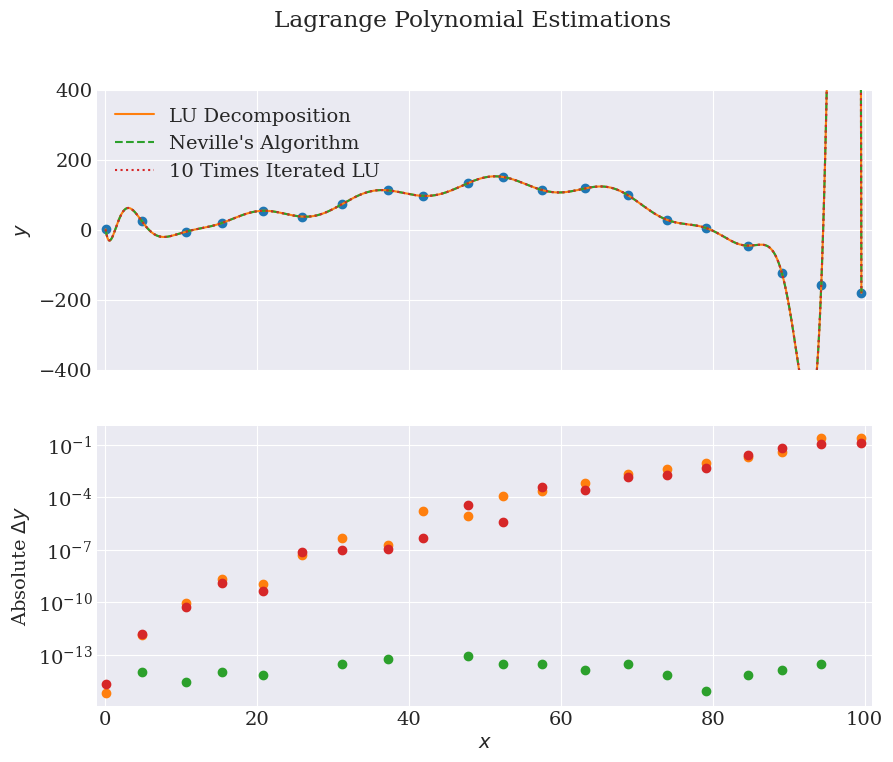
\includegraphics[width=\textwidth]{results/vandermonde_fitresults.png}
    \caption{Results of the polynomial estimations of the data. A full description of the algorithms and a full discussion of the text is given in text. \textit{top}: Provided twenty data points combined with the three estimated polynomials going through each of these points. \textit{bottom}: Logarithmic absolute difference between the estimated polynomials and the true data values evaluated at each $x_i$.}
    \label{fig:vandermonde_fitresults}
\end{figure}

Initially we can see that each of the three polynomials go through each of the twenty data points in almost exactly the same manner. It is impossible to see any difference by eye on a linear scale. However from the bottom panel we can see that there is a difference between the LU Decomposition and Neville's Algorithm method when evaluated at the $x_i$. The error for the polynomial interpolator is significantly lower for all $x$, and the error for the LU decomposition implementation increases of approximately thirtheen orders of magnitude throughout the entire dataset. Additionally we see virtually no improvement in error after attempting to iteratively improve the estimate with LU decomposition.
\\ \\
The consistently low values for absolute difference through Neville's Algorithm make sense due to the definition of the equation used for the estimations. Neville's equation is mostly based on the true values, $y_i$ and the distance between the corresponding $x_i$ and the point we want to interpolate. If that distance is very small, then the deviation from $y_i$ will by definition be very small as well. 
\\ \\
The pattern of increasing absolute difference in both LU decomposition implementations seems weird at first sight. But this most likely arises from the increasingly 'weird' behaviour of the polynomial that is clearly visible in the top panel. It has immensly steep slopes surrounding the final three data points, which means the estimation of a $y$ value can be very sensitive to a tiny variation in $x$, leading to larger uncertainties. The absence of any improvement for the iterated LU decomposition method could have arised from the large scale difference between the $y$ and $\Delta y$. After one iteration we already have a realtively good estimation which at its maximum has an uncertainty of $\sim 0.1$ on a value of $200$. Adding additional improvement with this iterative process just adds extra negligble terms that do not significantly change our estimations. We confirmed this by looking at the $\delta c$ for the last point, which are usually on the order of $\sim 10^{-3}$, too small to be noticed after ten iterations.

\subsection{Implementation Speed}

As a final comparison between each of the three methods we measure their execution times. To keep the run time of the complete assignment small we set a limit of one minute for this section, which allows 100 iterations of each algorithm. The results are presented in Table \ref{tab:vandermonde_timeit} and the associated code is presented at the end of this section.

\begin{table}[h]
    \centering
    \begin{tabular}{c|c}
        \hline
        \input{results/vandermonde_timetab.txt}
    \end{tabular}
    \caption{Runtime of each of the three algorithms described in the text expressed in milli-seconds, averaged over 100 iterations each.}
    \label{tab:vandermonde_timeit}
\end{table}

We see that the LU decomposition, while slightly less precise as we saw in the previous section, is faster than Neville's Algorithm by almost two orders of magnitude. Additionaly, we can very clearly see the fact that subsequent iterations of solving a system of linear equations with an LU matrix can be done very quickly. The LU decomposition iterated ten times is only $\sim 5$ times slower than the non-iterated version. However as we saw in the last section, in this specific case this additional computing time did not result in extra accuracy.

\lstinputlisting[caption={Code for the algorithm execution time estimation}, linerange={111, 137}]{vandermonde.py}
